\documentclass[b5paper]{book}
\usepackage[utf8]{inputenc}
\usepackage[T1]{fontenc}
\usepackage[english]{babel}
\usepackage[ddmmyy]{datetime}
\usepackage[chapter]{minted}
\usepackage{mdframed}
\usepackage{graphicx}
\usepackage{fancyvrb}
\usepackage{upquote}
\usepackage{xcolor}
\usepackage{amsmath}
\usepackage{subcaption}

\definecolor{folder}{HTML}{325fcf}
\setminted[latex]{frame=lines,linenos,autogobble}
\setminted[bash]{frame=lines,linenos,autogobble}
\newcommand{\ignore}[1]{} % Does nothing. \ignore{$} to trick highlighting.

\newcommand{\latexin}{\mintinline{latex}}
\newcommand{\latexone}{\mint[frame=none,numbers=none]{latex}}

\newcommand{\reflst}[1]{Listing~\ref{lst:#1}}
\newcommand{\reffig}[1]{Figure~\ref{fig:#1}}
\newcommand{\refch}[1]{Chapter~\ref{ch:#1}}
\newcommand{\refsec}[1]{Section~\ref{sec:#1}}
\newcommand{\reftab}[1]{Table~\ref{tab:#1}}

\renewcommand{\dateseparator}{.}

\title{Coding for Non-Coders}
\author{Sigvald Marholm}
\date{\today}

\begin{document}

\maketitle
\tableofcontents

\chapter{Introduction}
Programmers, engineers, scientists and tech-savvy people in general have had the opportunity to learn a bunch of different computer programs and programming languages which makes their everyday work in front of the computer both easier and more efficient. In comparison, less technically oriented people, who lack such a toolbox, often end up using inconvenient tools and therefore end up using inefficient and impractical solutions.

Consider for instance that you have hundreds of photos and you’d like to change the resolution on all of them? Or maybe add a watermark before sharing them? Or change the filename to include the date? Such tasks can be tedious if you don’t know the right tools. However, the file names of all files can be changed using a single command in the Bash command line interface. A script that adds a watermark to every image takes less then 20 lines of code using the Python scripting language. Of course, programming takes time to learn, and it’s not for everybody to become a full time professional programmer. But with the emergence of modern low-threshold scripting languages like Python, why should such handy techniques still be reserved for geeks only?

Another thing which many may benefit from is learning a professional typesetting tool like LaTeX to write documents. Applications, CV’s, reports, slideshows, etc. Because let’s admit it: Most of us aren’t typographists. We don’t know exactly which font to use, which size, which line spacing and which margins to use everywhere to make a document look professional. LaTeX takes care of all that for you, but then you need to tell LaTeX what’s supposed to be a chapter, what’s a new paragraph, and so on. And that’s done by coding. It doesn’t have to be that hard, to start a new chapter with the title “Introduction”, for instance, you simply type 

\latexone{\chapter{Introduction}}
And how do you generate a table of contents in LaTeX? Simple. Because LaTeX know what the chapters are, all you have to do is type:
\latexone{\tableofcontents}
where you want your table of contents.

And as a last example, have you ever had to collaborate with someone to write a document in a normal text processing tool such as Microsoft Word? Then you’ll know it’s a mess. No two people can edit the document at once, despite editing different parts of the file. Documents written in LaTeX, as well as programs written in languages such as Python can be efficiently shared amongs many users using a Version Control System (VCS) such as Git and everyone can work on it simultaneously without stepping on each other’s toes! VCSs like Git also allows you to backtrack the whole history of your documents in case you regret something you once did.

The aim of this little book is to provide the normal guy on the street with at least a small toolbox allowing him or her to work more efficiently. More in a similar manner as professionals. The tools presented are carefully selected because together, they form a minimal toolbox allowing the reader to use a computer in such a rich way. Moreover, they are considered to be more useful, versatile and simple to learn than other alternatives. Admittedly, we will only scratch the surface of all these tools. Just enough to get you started, with pointers of where to look for further information. True, it will not even cover the same depth as most beginner’s books, since it is not the aim of this book to turn you into a programmer. However, it is assumed that the reader, being a generation which has grown up with technology, is capable of finding his/her way around in simple graphical computer programs. Therefore this book will focus on the coding aspects, only providing pointers to which graphical programs may be useful (for instance to make figures in documents).

Finally, each part are self-contained and may be read independently of the other parts (although using Git is kind of meaningless without knowing some other coding).
\chapter{Command Line Interfaces: Handling Files Efficiently}\label{ch:bash}
% Goal: 10 pages

\section{Why bash?}
\index{bash}
\index{CLI}
\index{command line interface}
It seems that many people are a bit scared of the \emph{command line interface} (CLI). But the fact is that it's extremely useful to know just a little bit for a multitude of reasons. For one thing, some things are done much more efficiently in the command line. Knowing the command line also helps giving a better understanding of the compilation of \LaTeX{} documents when we get to \refch{latex}, while for the chapters on Python and Git it is just plain indispensable. Still, perhaps the most important reason to learn about the command line is that it shows up all the time, and knowing just a little bit about it makes you a lot more competent with computers.

\index{operating system}
\index{OS}
\index{POSIX}
\index{shell}
\index{Linux}
\index{Unix}
\index{OS X}
Linux and OS X are both operating systems (OS) which behaves in a manner similar to the older Unix operating system with respect to at least how commands look and how files are accessed. Such operating systems are often referred to as Unix-like systems or just *nix. To further ensure that they can use the same commands and as such many of the same command line tools, they have been standardized according to the POSIX standard. However, many different command line interfaces, or \emph{Unix shells} exist, which may be slightly different while still being POSIX-compliant, but the most common one is named \emph{bash}. It's been around since 89 and is still going strong.

\index{Windows}
Windows on the other hand, has its own command line which is non-POSIX compliant. Accordingly, this chapter first deals with bash for the Linux and OS X users, and subsequently with the Windows command line. Skip whichever doesn't fit.  More space is devoted to bash and the reader may also find that bash is presented more as a tool useful on its own, whereas the Windows command line is merely to facilitate what we'll cover in the rest of the book. This reflects how the command lines are typically used in their respective operating systems: bash is simply a more integral part of the workflow in Unix-like systems and comes with more powerful commands. However, Windows 10 now comes with the possibility to enable bash (still a beta feature in the time of writing) and hopefully Windows will become POSIX compliant in the future, rendering the twofold division of this chapter unnecessary.

\section{Which tools you need}
\index{terminal}
\index{console}
\index{Cygwin}
The command line is shipped with the operating systems (often named \emph{terminal} or \emph{console}) so you do not need to install anything. If you like to try out bash from Windows you can install Cygwin which is available here:

~\\
\urlone{http://cygwin.com}

\index{WSL}
or in Windows 10, enable the Windows Subsystem for Linux (WSL) and install bash. Neither Cygwin or WSL will be covered herein, though, so you will have to read about those elsewhere.

\section{The file system}
\index{file system}
In Windows, the file system starts on a given hard disk or partition, say \verb|C:\|, and from there on you may have folders such as \verb|C:\folder| and files in this folder such as \verb|C:\folder\file|. The hard disk or partition is the starting point for the rest of the file system, and you have one letter per hard disk or partition.

\index{root}
In Unix-like systems, the file system starts at a \emph{root} directory which we simply denote by \verb|/| (not to be confused with the \emph{root user} to be discussed in \refsec{bash:permissions}). We denote a folder in this root directory like this: \verb|/folder|, and a file inside this folder: \verb|/folder/file|. But we do not have anything like \verb|C:\|. 

We may very well have separate hard disks or partitions within Unix-like file systems, but the division is such that for instance one hard disk hold everything in the root directory, but as soon as you enter a particular folder, for instance \verb|/home|, you enter the \emph{mount point} of another hard disk meaning that everything in this particular sub-folder is located on that other hard disk.

Also note that Windows uses backslash whereas in Unix it's a forward slash. Unix-like systems also care about small vs. capital letters in file and folder names (it is \emph{case sensitive}).

In Linux, there is a very well defined set of folders which always exists in the root directory, and they all have a well defined purpose. The most important one for beginners, is \verb|/home|. This folder has one directory per user, so if your username is ``peter'' your \emph{home folder} would be \verb|/home/peter|. This is where you put all your stuff, kind of like ``My Documents'' in Windows except that you actually \emph{do} have all your personal files only in your home folder. Programs and system files are located outside \verb|/home| and you generally cannot change any files outside your home folder. One benefit of this is that it becomes a lot easier to copy all your personal files from one computer to another (e.g.\ to take backup) without including programs and system files.

\section{Linux and OS X}

\subsection{The prompt and commands}
\index{prompt}
\index{home folder}
When opening the command line in Linux or OS X, it typically looks something like this:
\begin{verbatim}
peter@laptop:~$
\end{verbatim}
and you can start typing your command after the dollar sign. This is known as the \emph{prompt}. Here, ``peter'' is the name of the user, while ``laptop'' is the name of the computer. The tilde (\~{}) indicates which folder you are currently on, which by default is your home folder. Tilde is a short way of saying ``home folder'' (e.g.\ \verb|/home/peter|). If Peter has a sub-folder named ``bills'' (\verb|/home/peter/bills|) and he were to enter that folder, the prompt could look something like this:
\begin{verbatim}
peter@laptop:~/bills$
\end{verbatim}
For simplicity we will from now on use only \texttt{\$} as short-hand for the prompt.

\index{command}
A command in bash is written in the following way:

\begin{verbatim}
$ command argument1 argument2
\end{verbatim}

\index{switch}
\index{flag}
\index{argument}
\verb|command| is here actually just the name of the program which we run, and it may take several \emph{arguments} which are just input we pass to it. It may also have \emph{switches} (also known as \emph{flags}) which turn on and off options. For instance if we want to use a switch called \verb|-s|, the command would look like this:

\begin{verbatim}
$ command -s argument1 argument2
\end{verbatim}
\index{syntax}
Such rules for how code is written (its ``sentence structure'') is often called \emph{syntax}. 

\subsection{Navigating}
\subsubsection{Present working directory (*nix only)}
First we need to be able to navigate around in folders in the command line. In bash, the prompt is customizable and sometimes do not display the full path, or ``present working directory''. To get it, type (you are encouraged to test out the commands as we go):

\index{\Verb+pwd+}
\begin{Verbatim}[commandchars=\\\{\}]
\$ pwd
/home/peter
\end{Verbatim}
Note that the second line does not have a prompt. This is the output from the command you entered, which is only \verb|pwd|. 

\subsubsection{List folders and files}\label{sec:bash:ls}
\index{\Verb+ls+}
To show all the files and sub-folders inside the present working directory you can use the ``list'' command \verb|ls|:

\begin{Verbatim}[commandchars=\\\{\}]
$ ls
file1  file2  \textcolor{folder}{folder1}  \textcolor{folder}{'folder 2'}
\end{Verbatim}
\ignore{$}
Clearly, this folder has two files and two folders. Most systems are configured to highlight the folders by some color. I recommend you create a folder named \verb|test| (not necessarily using the command line yet) containing some sub-folders and files like here which you can try out the commands on as we go.

To get a more detailed view, you can use the switch \verb|-l|:

\begin{Verbatim}[commandchars=\\\{\}]
$ ls -l
total 8
-rw-r--r-- 1 peter peter    0 2016-10-27 12:36 file1
-rw-r--r-- 1 peter peter    0 2016-10-27 12:36 file2
drwxr-xr-x 2 peter peter 4096 2016-10-27 12:36 \textcolor{folder}{folder1}
drwxr-xr-x 2 peter peter 4096 2016-10-27 12:36 \textcolor{folder}{'folder 2'}

\emph{
permissions  user  group size last-changed     name
}
\end{Verbatim}
\ignore{$}
Here we have added a brief description below each column. The last three are the size of the file in bytes, the date and time the document was last edited, and the name of the file or folder. We'll get back to the first three columns i \refsec{bash:permissions}. However, notice that the first character in the \emph{permissions}-string is ``d'' for folders/directories.

\begin{table}
	\centering
	\caption{Options for \texttt{ls}}
	\begin{tabular}{ll}
	\hline
	\verb|-a|		&	list all files (including hidden files starting with ``.'').	\\
	\verb|-h|		&	human readable file sizes (when using \verb|-l|)				\\
	\verb|-l|		&	long (detailed) listing										\\
	\verb|--help|	&	print a ``help'' section for this command
	\end{tabular}
	\label{tab:bash:ls}
\end{table}

In \reftab{bash:ls} there are some more options you can try out. To get a full overview of the functionality of \verb|ls|, you can write:

\begin{verbatim}
$ ls --help
\end{verbatim}

\index{\Verb+--help+}
\verb|--help| also works for many other commands, and adding \verb|--help| to a command should be your first attempt at figuring out how it works. Since ``help'' is a whole word rather than just a letter, the most common syntax is to use two dashes.

The options with a single dash, can often be combined. For instance, the following two commands are equivalent:

\begin{verbatim}
$ ls -l -h -a
\end{verbatim}
and

\begin{Verbatim}[commandchars=\\\{\}]
$ ls -lha
total 16K
drwxr-xr-x 4 sigvald sigvald 4.0K 2016-10-27 12:36 \textcolor{folder}{.}
drwxr-xr-x 7 sigvald sigvald 4.0K 2016-10-27 19:19 \textcolor{folder}{..}
-rw-r--r-- 1 sigvald sigvald    0 2016-10-27 12:36 file1
-rw-r--r-- 1 sigvald sigvald    0 2016-10-27 12:36 file2
drwxr-xr-x 2 sigvald sigvald 4.0K 2016-10-27 12:36 \textcolor{folder}{folder1}
drwxr-xr-x 2 sigvald sigvald 4.0K 2016-10-27 12:36 \textcolor{folder}{'folder 2'}
\end{Verbatim}
\ignore{$}
You can see that the file sizes is now specified in kilobytes due to \verb|-h| and in addition we got two more folders.

In Unix, folders and files starting with a period are \emph{hidden} and to show them we must use \verb|-a|. The folders \verb|.| and \verb|..| are special: \verb|.| is always the current folder (present working directory), while \verb|..| is the parent folder (one level up). Their usefulness will become more evident as we proceed.

\subsubsection{Change directory}
\index{\Verb+cd+}
Whenever you want to enter a folder, you use the ``change directory'' command, e.g.\ to enter \verb|folder1|:

\begin{verbatim}
cd folder1
\end{verbatim}
Most Unix-like systems features rich auto-completion, which means that after entering \verb|cd fo| you can hit tab and it automatically fills in \verb|cd folder|. Since it does not know whether you want to enter \verb|folder1| or \verb|folder 2| you will have to write the last part yourself. To go back (one level up), you can use the special name for the parent folder:

\begin{verbatim}
cd ..
\end{verbatim}

Notice that to enter \verb|folder 2|, you can not write

\begin{verbatim}
cd folder 2
\end{verbatim}
\index{escape}
since the computer will interpret this as a command having two arguments separated by a space: \verb|folder| and \verb|2|. Therefore, you must either \emph{escape} the space like this:

\begin{verbatim}
cd folder\ 2
\end{verbatim}
or enclose the argument in `` and '':

\begin{verbatim}
cd "folder 2"
\end{verbatim}

\index{absolute path}
\index{relative path}
Some further examples to test and expand your understanding can be found in \reftab{bash:cd}. Note that paths starting with the root directory (\verb|/|) or home folder (\verb|~|) renders to be the same file/folder no matter what your present working directory is. Such folders are coined \emph{absolute paths}, whereas paths which specifies a file relative to you present working directory are labeled \emph{relative paths}. The top four examples in \reftab{bash:cd} use relative paths while the remaining four use absolute paths. Beware, thought, that \verb|~| varies according to which user you are logged in as.

\begin{table}
	\centering
	\caption{Examples of \texttt{cd}.}
	\begin{tabular}{ll}
	\hline
	\verb|cd folder1/subfolder|	&	go to \verb|subfolder| inside \verb|folder1| inside this folder	\\
	\verb|cd ./folder/subfolder|	&	same as above		\\
	\verb|cd ..|					&	go to parent folder	\\
	\verb|cd folder/..|			&	stay at this folder	\\
	\verb|cd ~|					&	go to home folder 	\\
	\verb|cd ~/bills|			&	go to \verb|bills| inside home folder \\
	\verb|cd /|					&	go to root folder	\\
	\verb|cd /home/peter|		&	go to \verb|/home/peter| wherever you may already be
	\end{tabular}
	\label{tab:bash:cd}
\end{table}

\subsection{Creation and destruction}
To make a new directory \verb|newfolder| type:

\index{\Verb+mkdir+}
\begin{verbatim}
$ mkdir newfolder1
\end{verbatim}
you can also create several folders at once by passing several arguments to \verb|mkdir|:

\begin{verbatim}
$ mkdir newfolder2 newfolder3
\end{verbatim}
Similarly, new empty text files can be created using \verb|touch|:

\index{\Verb+touch+}
\begin{verbatim}
$ touch newfile1 newfile2 newfile3
\end{verbatim}
If the file already exists, \verb|touch| merely changes the ``last changed'' time to the current time (i.e.\ more like a gentle touch than actual editing). Use \verb|ls| to verify that the files and folders were indeed made.

\index{\Verb+rm+}
Files are delete/remove using \verb|rm|, which also takes an arbitrary number of arguments:
\begin{verbatim}
$ rm newfile1 newfile2 newfile3
\end{verbatim}
however, in this case it would be simpler to just write:
\begin{verbatim}
$ rm newfile*
\end{verbatim}
\verb|*| is a \emph{wildcard} which matches anything. Thus both \verb|newfile1|, \verb|newfile2| and \verb|newfile3| is matched by \verb|newfile*|. Wildcards can be very useful. Consider for instance that you'd like to remove all .txt files from a folder. You would simply navigate to that folder, and write:

\begin{verbatim}
$ rm *.txt
\end{verbatim}

Removing folders is done in a similar way, except that you must add the switch \verb|-r| which stands for ``recursive'':

\begin{verbatim}
$ rm -r newfolder*
\end{verbatim}
In this context ``recursive'' simply means it will also remove the contents within the folders. Beware that \verb$rm$ do not ask if you are sure before it deletes something. If you've managed to write the command correctly, it assumes that you are sure, and it will be properly deleted, i.e.\ not put in a trash bin.

\subsection{Copying, moving and renaming}
\index{\Verb+cp+}
\index{\Verb+mv+}
\verb|mv| and \verb|cp| are used to moving and copying files and folders, respectively, and have similar syntax which is:

\begin{verbatim}
$ mv <source> <destination>
\end{verbatim}
or
\begin{verbatim}
$ cp <source> <destination>
\end{verbatim}
where \verb|<source>| is the file(s) to be moved or copied, and \verb|<destination>| is where it should be moved or copied to. As usual, these can be specified using both absolute or relative paths. For example to move \verb|file1| to \verb|folder1|:

\begin{verbatim}
$ mv file1 folder1
\end{verbatim}
and to move it back to this folder:

\begin{verbatim}
$ mv folder1/file1 .
\end{verbatim}

To move \verb|file1| to the parent folder, you could either do like this:
\begin{verbatim}
$ mv file1 ..
\end{verbatim}
or you could step out of the current folder (presumably named \verb|test|) using \verb|cd| first and do like this:
\begin{verbatim}
$ cd ..
$ mv test/file1 .
\end{verbatim}
How would you go about to move \verb|file1| to your home folder? Try it out!

Note that when \verb|<destination>| is a folder, the file is simply moved to that folder. If \verb|<destination>| is a non-existing file name, however, the file is given that name. Therefore, \verb|mv| is used both for moving \emph{and} renaming files. For instance, here \verb|file1| is given the new name \verb|newname|:

\begin{verbatim}
$ mv file1 newname
\end{verbatim}
while here, it is given a new name and moved inside \verb|folder1| in one go:

\begin{verbatim}
$ mv file1 folder1/newname
\end{verbatim}

Like with the arguments of \verb|rm|, \verb|<source>| could actually be a list of several files or wildcards could be used. For instance, to move both \verb|file1| and \verb|file2| to \verb|folder1|:

\begin{verbatim}
$ mv file1 file2 folder1
\end{verbatim}
or equivalently
\begin{verbatim}
$ mv file* folder1
\end{verbatim}
In this case, however, \verb|<destination>| has to be a folder since \verb|file1| and \verb|file2| cannot both be renamed to the same file name. 

In all these examples, \verb|cp| could have been used in place of \verb|mv| to leave a copy of the original file. Go through the examples again and make sure you understand what would happen if you used \verb|cp|.

\verb|mv| and \verb|cp| could also be used to move, rename or copy whole folders. For instance to rename \verb|folder 2| to \verb|folder2| (without space):

\begin{verbatim}
$ mv "folder 2" folder2
\end{verbatim}
As you would expect, it's similar to renaming/moving files. \verb|cp|, though is slightly different. To make a copy of \verb|folder2| named \verb|folder3|:

\begin{verbatim}
$ cp -r folder2 folder3
\end{verbatim}
Like with \verb|rm|, we need to tell \verb|cp| to also copy the contents of the folder (including other folders and their contents) using the recursive option. Otherwise \verb|cp| will ignore the folder. The logic behind this is that with \verb|mv| you're kind of just renaming the outermost folder, leaving everything inside it as it is, and therefore you do not need the recursive option.

\subsection{Advanced example: renaming}
To illustrate the power of the command line, consider that you have a folder from a digital camera. Most of the files are images whose names end with .JPG, but some are movies ending with .MPG. What if you want to sort out the movies from the images and store them in separate sub-folder named \verb|images| and \verb|movies|? (I'm not suggesting this is neither a good nor a bad idea. It's just an example). Then you can navigate to the image folder and do something like this:

\begin{verbatim}
$ mkdir movies images
$ mv *.MPG movies
$ mv *.JPG images
\end{verbatim}
Done! Beat this in the graphical interface. Make sure you understand this example.

\index{\Verb+rename+}
\verb|mv| is great for most purposes, but as pointed out earlier, you cannot \emph{rename} multiple files at once using it since they all have the same \verb|<destination>|. \verb|rename| is a tool which can rename multiple files at once by using pattern-matching, it has the following syntax:

\begin{verbatim}
$ rename <expression> <replacement> <files>
\end{verbatim}
In our example, we have bunches of files with suffix .JPG. Now we'd like to rename all of them to .jpg because .JPG is ugly. Then .JPG is the ``expression'' we wish to ``replace'' by .jpg in all files ending with .JPG in the folder \verb|images|. Accordingly:

\begin{verbatim}
$ cd images
$ rename .JPG .jpg *.JPG
\end{verbatim}
We could do likewise for the .MPG files.

Next, let's assume we'd like to append the current date, \verb|2016-10-28-| to the beginning of the name:

\begin{verbatim}
$ rename "" 2016-10-28- *.jpg
\end{verbatim}
here, the expression to match is empty (only enclosed by quote marks), which makes us get a match immediately (at the beginning of the name) where we insert the replacement.

\subsection{View and edit text files}
Viewing text files in bash is straight forward, but there exists a bunch of different viewers (and editors). Some of the most common ones and how they differ are listed in \reftab{bash:editors}. To use one of them, simply type its name followed by the file to view, e.g. to use \verb|cat| to view \verb|document.txt|:

\index{\Verb+cat+}
\index{\Verb+more+}
\index{\Verb+less+}
\index{\Verb+head+}
\index{\Verb+tail+}
\begin{verbatim}
$ cat document.txt
\end{verbatim}
Find (or create) some plain text file (e.g.\ not a full MS Word document but typically something ending with .txt) and try out the programs listed in \reftab{bash:editors}. A document is a bit like a cat. Do you want to print only the \verb|head| or the \verb|tail|? Or perhaps you want to print \verb|more|? How about the whole \verb|cat|? And remember, \verb|less| is more.

\begin{table}
	\centering
	\caption{Text viewers and editors}
	\begin{tabular}{ll}
	\hline
	\verb|cat|		&	Print the whole file to terminal at once 	\\
	\verb|head|		&	Prints the first part (head) of a file \\
	\verb|tail|		&	Prints the last part (tail) of a file	 \\	
	\verb|more|		&	Print file bit by bit (scrolling down) as you press enter	\\
	\verb|less|		&	Like \verb|more| but also allows you to scroll back up\\& (less is more). Quit using q. \\	
	\hline
	\verb|nano|		&	Full editor \\
	\verb|vi|		&	Full editor
	\end{tabular}
	\label{tab:bash:editors}
\end{table}

\subsubsection{Nano}
\index{Nano}
\index{\Verb+nano+}
Two full editors which also allows editing the documents are presented in this list. \emph{Nano} is the simpler one of the two and it basically behaves how you would expect, perhaps except that you have to navigate using the arrows instead of the mouse. At the bottom of the program, there's a list of shortcuts which is reproduced here in \reffig{bash:nano}. For the instance the shortcut \verb|^X| means that you can hit Ctrl+X to exit Nano. The \verb|^| character means ``Ctrl+''. Next, Nano may ask if you want to save your changes, and you answer simply by pressing Y or N. At all times, Nano will maintain a list of available control keys at the bottom so you don't really have to remember anything.

\begin{figure}
	\centering
	\includegraphics[width=\textwidth]{graphics/nano.png}
	\caption{Nano shortcut list}
	\label{fig:bash:nano}
\end{figure}

\subsubsection{Vim}
\index{Vim}
\index{Vi}
\index{\Verb+vi+}
The other editor is an old classic named \emph{Vi}, or actually we're going to use an improved version of Vi named \emph{Vi Improved} (Vim). On most systems Vim and not Vi is what shows up when you use the command \verb|vi|. While Vim is a very powerful and convenient editor once you're used to it, it's not at all intuitive, and many users otherwise familiar with the command line suddenly feel helpless once a file is opened in Vim. In fact, the only reason such a ``difficult'' editor is presented here, is because you're likely to stumble upon it.

Vim operates with different \emph{modes}. Initially, you'll be in \emph{command mode} (see \reffig{bash:vi}) where the letter keys are not used to write text into the document, but rather acts as shortcuts to do various operations (a better name would perhaps have been \emph{shortcut mode}). To enter the \emph{insert mode}, press Insert and the text \verb|--INSERT--| shows up in the last line in the window. Now you can edit text similarly as in Nano. Hitting Insert again makes you toggle between insert and \emph{replace mode} (where you what you type replaces existing text). To get back to (the default) command mode, hit Esc. Now to quit Vim, you first need to enter \emph{last line mode} by typing colon (\verb|:|) while in command mode. In last line mode, you can type short commands to save the document, quit Vim, and so on (actually I would've preferred if \emph{this} was named command mode). The most important commands are listed in \reftab{bash:vi}. Try to open, edit, save and quit a document using Vim. If you don't like it, feel free to use Nano or a graphical editor instead. It's just nice to be aware of Vim.

\begin{table}
	\centering
	\caption{The most important Vim last line commands}
	\begin{tabular}{ll}
	\hline
	\verb|q|			&	Quit (only if all changes are saved)	\\
	\verb|q!|		&	Force quit (discard unsaved changes)	\\
	\verb|w|			&	Write to file (save)					\\
	\verb|wq|		&	Write and quit
	\end{tabular}
	\label{tab:bash:vi}
\end{table}

\begin{figure}
	\centering
	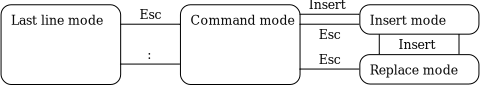
\includegraphics[scale=0.8]{graphics/vi.pdf}
	\caption{Vim modes}
	\label{fig:bash:vi}
\end{figure}

\subsection{Permissions}\label{sec:bash:permissions}
\index{permissions}
\subsubsection{Users and groups}
\index{users}
\index{groups}
About time to get back to the first columns we get when using \verb|ls -l| (see \refsec{bash:ls}). In Unix-like systems, there are \emph{users} (e.g.\ ``peter'') and \emph{groups}, and each user may belong to multiple groups. Indeed, you may feel that you only need one user on your own personal computer, but most operating systems support computers, or networks of computers, with multiple users. In many offices, for instance, users log on to a network where their user is only one of many.

\index{\Verb+groups+}
To see which groups you belong to is simple:

\begin{verbatim}
$ groups
\end{verbatim}

Anyhow, each file is owned by one user, and is associated with one group. The owner of the file is the second column in the output of \verb|ls -l| while the group is the third. Normally, there exists a group with the same name as the user, and this group only has that user as a member. E.g. there is a group ``peter'' which only has the user ``peter'' as its member. This is useful when you don't really want a file to belong to any other groups but yourself. By default you will be the owner of all files you create, and the associated group is the group consisting only of you.

The owner may have different permissions than the other members of the group. For instance, maybe you want to share some information stored in a text file with a bunch of people who you collaborate with in a top secret project, but you don't want them to be able to edit its contents on behalf of you. In this case, a group would be made for the members of the project, and that group would be given \emph{reading} permission only. The owner, you, would have both \emph{reading} and \emph{writing} permission. Since the project is top secret, users who do not belong to the group don't have any permissions.

\index{symbolic link}
\index{flag}
The first column in the \verb|ls -l| output is a string of \emph{flags}, that is, options which can either be on or off, which decides which permissions different categories of users have. If all flags are on, the string of flags looks like in \reffig{bash:permissions}. The first letter is not strictly speaking a permission flag, but it is \verb|d| if the item is a directory or \verb|l| if it is a \emph{symbolic link} (or \emph{shortcut} in Windows terminology). It may also be \verb|s| or \verb|t| but we won't cover those here. For most files, it is just \verb|-|.

\begin{figure}
	\centering
	\includegraphics[width=0.3\textwidth]{graphics/permissions.pdf}
	\caption{Permission flags}
	\label{fig:bash:permissions}
\end{figure}

Further on, there are three blocks of the three letters \verb|rwx|. The first block indicates the permission of the \emph{user} who owns the file, the second block indicates the permissions of the members of the \emph{group} associated with the file, while the third indicates the permission of \emph{others} who aren't even members of the group. \verb|r| indicates that \emph{reading} is permitted, \verb|w| indicates \emph{writing} is permitted while \verb|x| indicates \emph{executing}, i.e.\ running the file as a program is permitted. The ``execute'' flag should be on only for programs and folders. For folders it allows the user to open the folder. A deactivated permission is replaced by a dash.

To make a few examples, the text file in the top secret project would have permission mode \verb|-rw-r-----|. A folder would typically be \verb|drwxr-xr-x| which means that all users can open (execute) it and read its contents but only the owner can add files to it. Whether users can read the files within it depends on the permission mode of \emph{those} files.

\subsubsection{The superuser}
\index{superuser}
\index{root}
Normal users mostly have only reading permission outside their own home folder. This means you can run all the programs installed on your computer, but you cannot tinker with it. It also prevents malicious software from infecting your system through your user since your user cannot grant it permission to the system files. This is one of the reasons why Unix systems are generally regarded more safe than Windows, although Microsoft lately has become better at not letting users permanently run the Administrator user.

\index{\Verb+sudo+}
On all Unix systems there is a superuser named \emph{root} (not to be confused with the \emph{root directory}). This user has the special privilege that it can do anything. It is similar to \emph{Administrator} in Windows systems, but is even more powerful. You normally cannot log in to this user, but if you are on the \emph{sudoers list} you are kind of regarded as a system administrator and are allowed to run one command at a time as root by using the ``superuser do'' command \verb|sudo|. To illustrate, one could go to a folder you do not have write permission to (e.g.\ \verb|/etc|) and try to create a new file:

\begin{verbatim}
$ cd /etc
$ touch newfile
touch: cannot touch 'newfile': Permission denied
\end{verbatim}
However, the superuser can do it for you if you are on the sudoers list:

\begin{verbatim}
$ sudo touch newfile
\end{verbatim}
Normally you would be on the sudoers list on your own personal computer, but in larger networks (e.g.\ offices) this privilege would be restricted to the system administrators only. Be careful when using \verb|sudo|. Don't run software you don't know what is using the superuser.

\subsubsection{Changing permissions}
\index{\Verb+chmod+}
Now that we know what it all means, it's time to learn how to change permission. Changing permission mode can be done with \verb|chmod|:

\begin{verbatim}
$ chmod <changes> <file(s)>
\end{verbatim}
where \verb|<changes>| specifies which changes should be made to the permissions of the file(s). This can be specified in several different ways, but knowing one is sufficient. Changes can be specified as three symbols according to \reftab{bash:chmod}. For instance, to add write permission to the group of \verb|file1| and then remove the read permission of ``others'' can be done by two consecutive calls to \verb|chmod|:

\begin{verbatim}
$ chmod g+w file1
$ chmod o-r file1
\end{verbatim}
You may want to call \verb|ls -l| at this point to verify that the permission mode is what you expect.

\begin{table}
	\centering
	\caption{Permission modes for \texttt{chmod}}
	\begin{tabular}{ll|ll|ll}
	\hline
	\multicolumn{2}{c}{First letter(s)} & \multicolumn{2}{|c|}{Middle letter}  & \multicolumn{2}{c}{Last letter(s)}  \\
	\hline
	\verb|u|		&	User		& \verb|+|	& Add		& \verb|r|	& Read		\\
	\verb|g|		&	Group	& \verb|-|	& Remove		& \verb|w|	& Write		\\
	\verb|o|		&	Others	& 			&			& \verb|x|	& Execute	\\
	\verb|a|		&	All		&			&			&			&
	\end{tabular}
	\label{tab:bash:chmod}
\end{table}

Note that several letters from the first or last column of \reftab{bash:chmod} can be combined. To exemplify, let's add read and execute permissions to \verb|file1| and \verb|file2| for all users (the owner, the group members and others):

\begin{verbatim}
$ chmod a+rx file*
\end{verbatim}

At last, changing group and owner can be done by the following commands:

\index{\Verb+chown+}
\index{\Verb+chgrp+}
\begin{verbatim}
$ chgrp <group> <file(s)>
$ chown <owner> <file(s)>
\end{verbatim}
Changing permission mode and group can only be done by the owner and root, while changing owner can only be done by root. Thus you will get a ``permission denied'' message when trying to change owner unless you do:

\begin{verbatim}
$ sudo chown <owner> <file(s)>
\end{verbatim}

Often you do not need to bother too much about the permission flags, but once in a while you get an error such as ``Permission denied'' and now you know that you can fix it either using \verb|chmod| or \verb|sudo|. Nobody goes around remembering exactly how all commands work. The important thing is to know what is possible and where to figure out how to use it when you need it.

\subsection{Advanced example: backup}
\index{backup}
\index{\Verb+rsync+}
We have seen how to use \verb|cp| which is excellent for small copying tasks. One operation which is dreaded by most people, though, is taking backup of large folders. All of a sudden maybe there's a file which couldn't be read. You deal with the file somehow and start again, but then you get asked a thousand times if you're sure you want to overwrite the files you successfully copied there the first time around. For such things, \verb|rsync| is perfect.

Unlike copying in the graphical user interface, \verb|rsync| does not stop every time a single file couldn't be copied. It just prints an error and proceeds. Moreover, if the copying is interrupted, it will proceed where you left of the next time you run the command. It's even able to proceed midways in a file if you're copying big files. \verb|rsync| has a similar syntax as \verb|cp|:

\begin{verbatim}
$ rsync <source> <destination>
\end{verbatim}
\index{mount}
Let's say we want to copy all your personal files, which on Unix-like systems usually is limited to your home folder. By only copying the home folder we avoid copying a bunch of program and system files. We'd like to copy them to an external hard drive, which on Unix-like systems is \emph{mounted} as a folder. To make sure it is mounted, you can simply open it in the graphical user interface, and find its path there. You can also try to figure out how to use the commands \verb|mount| and \verb|umount|, which are not covered here.

Let's assume your drive is mounted to \verb|/media/mydrive| and that you've created a folder \verb|/media/mydrive/backup| which is the destination of your backup. The source is \verb|~/*|, everything in your home folder. To copy folders, we need to include the recursive switch \verb|-r|. Then a correct way to do this operation would be:

\begin{verbatim}
$ rsync -r ~/* /media/mydrive/backup
\end{verbatim}
However, \verb|rsync| by default doesn't say much, so after a few hours maybe we'll start wondering if anything is actually happening. By using the \verb|-v| switch we make \verb|rsync| more \emph{verbose} (talkative), such that we can see which file it's currently copying. But then, if you leave your computer maybe for hours, you're unlikely to spot which files couldn't be copied.

\subsubsection{Redirecting output}
\index{standard output}
\index{standard error}
\index{output redirection}
Everything which is output to terminal is output in one of two ways: Either, it's \emph{standard output}, which covers most of what you see, or if something goes wrong, it's \emph{standard error}. It's possible to \emph{redirect} either output such that it's not printed to the terminal but instead to a text file using any of the operators listed in \reftab{bash:redirection}. For our case, we may like to view the progress on screen but to filter out all errors to a text file so we can go through them afterwards. Then, we could write:

\begin{verbatim}
$ rsync -rv ~/* /media/mydrive/backup 2>> errors.txt
\end{verbatim}
If the copying is interrupted, and we run the command again the second run will not delete the contents already in \verb|errors.txt| since we used the ``appending'' operator. Of course, redirecting the output to a file works with any command.

\begin{table}
	\centering
	\caption{Output redirection}
	\begin{tabular}{ll}
	\hline
	\verb|>|		& Redirect standard output to file (overwrite if file exists)	\\
	\verb|>>|	& Redirect standard output to file (append if file exists)	\\
	\verb|2>|	& Redirect standard error to file	 (overwrite if file exists)	\\
	\verb|2>>|	& Redirect standard error to file	(append if file exists)	\\
	\verb|&>|	& Redirect both to file (overwrite if file exists) \\
	\verb|&>>|	& Redirect both to file (append if file exists) \\
	\verb$|$		& Redirect output to input of another program \\
	\end{tabular}
	\label{tab:bash:redirection}
\end{table}

\verb|rsync| can also be used to copy files from/to another computer across a network, among other things, but that's something you can read about somewhere else whenever you need it.

\subsection{Executing programs and scripts}
Most of the commands you type into bash is actually a tiny program which resides in a special folder where bash looks for them (a few are built into bash). However, you can also run programs residing in other folders, but then you must include the path of the program. For instance, if you program is a file named \verb|program|:

\begin{verbatim}
$ /home/peter/program argument1 argument2
\end{verbatim}
Alternatively, you can navigate to the folder where \verb|program| lies and write:

\begin{verbatim}
$ ./program argument1 argument2
\end{verbatim}
Note that omitting \verb|./| will not work although it's a perfectly legitimate relative path.

One common pitfall you should be aware of is that the executable flag of \verb|program| must be set or you will get ``permission denied''. Setting the executable flag to programs and scripts is perhaps the most frequent use of \verb|chmod|. See \refsec{bash:permissions}.

\subsubsection{Bash scripting}
\index{script}
It is also possible to write \emph{bash scripts} which are small program snippets written in bash, typically stored in files ending with .sh. We will only skim the surface of shell scripting here, and you are not expected to be able to write your own scripts afterward. You can learn Python in \refch{python} which is both easier, more powerful and more versatile. However, it can be instructive just to see an example of how a bash script is written.

\index{shebang}
We'll proceed with our backup example, and make a file called \verb|backup.sh| which makes backups for you using \verb|rsync|. The script can be seen in \reflst{bash:script}. The first line is known as a \emph{shebang} (since it starts with a ``hash'' and a ``bang''/exclamation mark character) and simply tells the shell that this is a bash script. Following this, you can write bash commands as usual, and when the script is executed, bash will run one command after the other.

\begin{listing}
	\begin{minted}{bash}
		#!/bin/bash

		echo "Creating new backup"
		DATE=$(date +%Y-%m-%d)
		mkdir /media/mydrive/backup/$DATE
		rsync -rv ~/* /media/mydrive/backup/$DATE \
			2>> /media/mydrive/backup/$DATE-errors.txt
	\end{minted}
	\caption{A small bash script}
	\label{lst:bash:script}
\end{listing}
The first command we encounter, \verb|echo|, simply outputs a message to the screen. Next, we create a \emph{variable}, which just holds some text. Creating a variable can done be like this:

\begin{verbatim}
TEXT="Some text"
\end{verbatim}
After the variable is defined, you could use the variable as \verb|$TEXT| in all following commands, and it would be replaced by ``Some text''. The script is somewhat more complex. The following command is used to get the current date:

\begin{verbatim}
$ date +%Y-%m-%d
2016-10-31
\end{verbatim}
This command is written inside \verb|$(...)| which evaluates/runs the command and returns the output as text which is then stored to the variable \verb|$DATE|. Next we create a new backup folder for that date (e.g. \verb|/media/mydrive/backup/2016-10-31|) and use \verb|rsync| to take a backup of our home folder to that folder. If anything goes wrong, it is stored to a text file, e.g. \verb|/media/mydrive/backup/2016-10-31-errors.txt|. Line 6 was too long so we split it into two by escaping the character with a \verb|\| symbol.

Finally, we must set the execute flag to make it an executable and we can run it like any other program:
\begin{verbatim}
./backup.sh
\end{verbatim}

To make a more serious backup script, perhaps we would make sure the external hard drive was mounted first by running \verb|mount|. \verb|rsync| also supports \emph{incremental backup}, which is a clever way of only copying what has changed since the last backup. We will not delve into that, but the script provided herein could certainly be a starting point you could further expand on your own.

\subsection{Installing programs}
Most Unix based operating systems has a package system where you can install the vast majority of the software you'll ever need. The advantage of such a system over downloading executable files from an unknown web page is that there's a community which maintains a list of packages. The list consists of well known software that the maintainers approve. This makes it very unlikely that you'll ever get malicious software from the package system. Yet a reason why Unix-like systems are traditionally regarded as safer than Windows by many. You are encouraged to learn the most basic commands for the package manager on your system.

\subsubsection{Ubuntu, Mint and Debian-based Linuxes}
On Debian-based Linuxes such as Ubuntu and Mint, the package manager is called \verb|apt| and the syntax to download and install packages are:

\begin{verbatim}
$ sudo apt-get install <package(s)>
\end{verbatim}
\verb|sudo| is necessary since software will be installed on your system. Since the package manager is regarded as safe you do not have to worry about using \verb|sudo| to install software through \verb|apt-get|. You can also search for packages like this:

\begin{verbatim}
$ apt-cache search <keyword>
\end{verbatim}

\subsection{Advanced example: ImageMagick}\label{sec:bash:imagemagick}
\index{ImageMagick}
If you want to do something to many files (\emph{batch processing}), chances are its better to figure out a way to do it in the command line. You may have to search the web to find the right tools, since it is impossible to cover everything you might need in a small book (or any book for what matters). We'll cover one more such tool as an example, however.

Maybe you wouldn't think about editing images in the command line, but some editing is just incredibly convenient to do in the command line using a tool named ImageMagick. ImageMagick can be installed on Linux, OS X \emph{and} Windows, but is often pre-installed in Linux (TBD).

\subsubsection{Auto-crop}
Consider that you've made an illustration for a document such as the one depicted in \reffig{bash:trim}, but the program left out a large white area around it which you want to get rid of. This is easy using ImageMagick's command \verb|convert|:

\index{\Verb+convert+}
\begin{verbatim}
$ convert -trim before.png after.png
\end{verbatim}
The result can be seen in \reffig{bash:trim}. It couldn't have been simpler.

\index{\Verb+mogrify+}
The command \verb|mogrify| works in exactly the same way as \verb|convert| except that it can take many files, for instance to do this to all .png files in a folder:

\begin{verbatim}
$ mogrify -trim *.png
\end{verbatim}
Beware, though, that \verb|mogrify| replaces the original images so you may want to make a copy of them before running \verb|mogrify|.

\begin{figure}
	\begin{minipage}[b]{0.5\linewidth}
		\centering
		{%
			\setlength{\fboxsep}{0pt}%
			\fbox{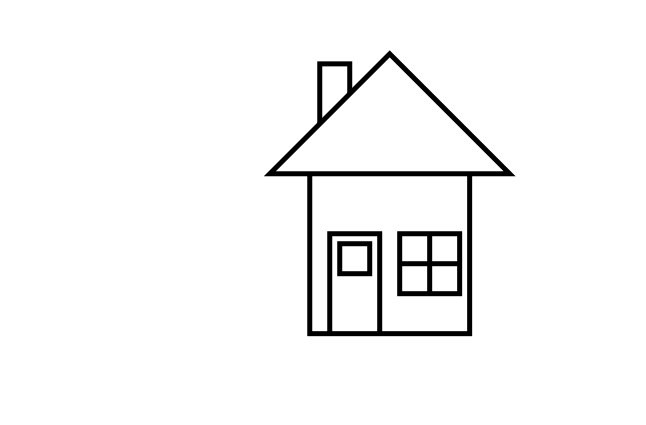
\includegraphics[scale=0.3]{graphics/trim_before.png}}%
		}%
		\subcaption{\texttt{before.png}}
	\end{minipage}%
	\begin{minipage}[b]{0.5\linewidth}
		\centering
		{%
			\setlength{\fboxsep}{0pt}%		
			\fbox{\includegraphics[scale=0.3]{graphics/trim_after.png}	}%
		}%
		\subcaption{\texttt{after.png}}
	\end{minipage}%
	\caption{Before and after trimming using ImageMagick}
	\label{fig:bash:trim}
\end{figure}

\subsubsection{Compressing images}
Another useful thing is to compress images. Consider for instance that you have a folder with a bunch of .jpg images, and you'd like to make thumbnails of them. You figure out that you want to reduce the JPEG quality factor to 85 (this is a number between 0 and 100, higher number means higher quality but also larger files) and reduce the width and height to 10\%. Then:

\begin{verbatim}
$ mkdir thumbnails
$ cp *.jpg thumbnails
$ mogrify -quality 85 -resize 10% thumbnails/*
\end{verbatim}
Note that since \verb|mogrify| overwrites its input files we created a new folder and copied all the images there before converting them. Another thing which is new to us, is the options may require additional inputs, e.g.\ here, the option \verb|-quality| takes the \emph{option argument} 85. Such an operation can reduce the file size by a factor of 100.

ImageMagick comes with a plethora of options, and you would simply have to look for them when you need them.

\subsection{The way forward}
The most important step forward, is perhaps to start actually using the command line. Sure, for browsing folders you will still likely just use the graphical interface, but whenever you're faced with, for instance the task of moving or renaming multiple files, you know it's simply more efficient in the command line. You may have to look up the commands, and you may feel a bit uncomfortable at first. But as time goes by, you will gradually become more confident. As you do, I encourage you to keep figuring out how to do stuff.

Some things we didn't have time to cover are the following commands: \verb|ps|, \verb|kill|, \verb|killall|, \verb|df|, \verb|grep| and the character \verb$|$. We also did not cover how to log into remote machines using the Secure Shell (SSH) protocol and to transfer files to/from such machines using Secure File Transfer Protocol (SFTP). The command line program ImageMagick is worth checking out if you deal a lot with images. In ImageMagick you can resize and compress all image files in a folder at once, along with a bunch of other things.

\subsubsection{OS X}
TBD. How do this work?

\subsection{``Executing'' programs}
ps, kill, killall

\subsection{Various useful commands}
df, ipconfig/iwconfig/ifconfig, etc.

\subsection{Advanced topics (if enough space)}
grep, rsync, imagemagick, |, >, >>, ls -l | more, sudo apt-get install

\subsection{Further studying}
Mention use of sftp, ssh and rsync through such protoccols. 

\section{Windows}

\subsection{Prompt and command}

In Windows, the prompt typically looks like this:
\begin{verbatim}
C:\>
\end{verbatim}
and if you enter ``My Documents'':
\begin{verbatim}
C:\My Documents>
\end{verbatim}

The Windows command line pretty much has the same syntax, but the name of the commands, what they do, what their arguments are and what their switches are is often different. One difference in syntax, though, is that switches are often (but not always) preceded by \verb$/$ rather than \verb|-|:

\begin{verbatim}
> command /s argument1 argument2
\end{verbatim}
This is inherited from the old operating system DOS.

Throughout the rest of the chapter, Windows commands will be written in parenthesis behind the bash commands whenever an equivalent exists.


\subsection{Listing files and folders}
In Windows, the \verb|dir| command is used to list the files and folders (directories):

\begin{Verbatim}[commandchars=\\\{\}]
> dir
2016-10-27 12:36  <DIR>      .
2016-10-27 19:19  <DIR>      ..
2016-10-27 12:36         0   file1
2016-10-27 12:36         0   file2
2016-10-27 12:36  <DIR>      folder1
2016-10-27 12:36  <DIR>      folder 2
\end{Verbatim}
\verb|<DIR>| indicates that the item is a directory and the numbers shown are the last changed date and the size in of the file in bytes, respectively.

To find more information about \verb|dir|, run:

\begin{verbatim}
> dir /?
\end{verbatim}
\verb|/?| is the Windows analogue to \verb|--help| in Unix-like systems. There is no analogue to the home folder in Windows.

\subsection{Change drive (Windows only)}
To change hard disk (partition) in Windows, e.g. from \verb|C:| to \verb|D:|, simply type:

\begin{verbatim}
> D:
\end{verbatim}

There are other books which provide much more details about these topics. However, it is not the aim of this book to give exhaustive knowledge about any topic, but merely a taste of what's possible within a few carefully selected topics. Hopefully, this is enough to provide a broad base, making the reader capable of expanding his/her knowledge using other resources (e.g.\ the internet) whenever needed. It's impossible to know in advance what one will need. Big books cover all you need plus a lot you'll never need. Indeed, the level of details in such books may be suitable for computer scientists. This book tries to cover \emph{less} than you need, but in such a way as to make you self-going. This makes a small book.
\chapter{Scripting: Automating Small Tasks}
60 pages
\section{Why Python?}
\section{Which tools you need}

\begin{enumerate}
	\item IPython and running scripts
	\item Variables (int,float,char) and operators
	\item Writing to display
	\item Lists and strings
	\item Input arguments
	\item Example: Computing cost of building something
	\item Conditionals
	\item Assignment: Can you afford building something
	\item Loops
	\item Functions
	\item Reading/writing files
	\item Example and Assignment: Todo-list handler
	\item Libraries and namespaces
	\item Example: Plot mathematical functions
	\item Assignment: Plot interest rates
	\item Example: Add watermark to images
	\item Assignment: Make images grayscale
	\item Example: Plotting image histogram
	\item Objects
	\item Further reading and topics
\end{enumerate}
\chapter{\LaTeX: Making Beautiful Documents}\label{ch:latex}
40 pages

\section{Why \LaTeX?}
\index{latex}
\index{WYSIWYG}
Most people need to write text documents from time to time, be it a CV, an article or a school assignment. Especially if you're writing something you'll use in your profession, you likely want it to \emph{look} professional which usually is not the case when you use tools like Microsoft Word or LibreOffice Writer. With these what-you-see-is-what-you-get (WYSIWYG) tools, the author spends time manually tweaking how stuff looks; where the title is, which fonts to use, text sizes, and placement. Most of us are not interested enough in typography to do this right. In comparison, using \LaTeX{}, the writer focuses on what stuff \emph{is}, rather than how stuff \emph{looks}. By telling \LaTeX{} ``this is a title'', or ``this is a new paragraph'' \LaTeX{} itself will figure out the proper formatting. It may seem unfamiliar at first that \LaTeX{} decides how stuff looks, indeed many novices try to force \LaTeX{} to display stuff in a particular way. My advice: don't!

\LaTeX{} certainly comes with a higher learning barrier before you can use it than WYSIWYG tools, but once you get familiar with it, I think you'll find that using it actually isn't that much slower, and it produces much better results. You may find a shift in what you spend time on: less time manually placing stuff, more time looking for how to do ``this thing'' with \LaTeX{} on the internet.

Other professional typesetting tools exist as well, but \LaTeX{} is very well developed and by far the most widespread, at least in scientific publications and books. We'll also see how to use it for making slideshow presentations, thus replacing tools such as Microsoft PowerPoint. If there's one typesetting tool you want in your toolbox to it's definitely \LaTeX{}.

\section{Which tools you need}
\index{highlighting}
\index{Texmaker}
\LaTeX{} can be written in any plain text editor (like Notepad if you're using Windows) and stored to a file ending with .tex. The .tex file is then \emph{compiled} to generate a .pdf-file using the command line tool \verb|pdflatex|. However, most users prefer a more specialized text editor which runs \verb|pdflatex| for you. Most such editors also supports highlighting, i.e.\ the application of different colors to different parts of the code to make it more readable. Many good editors exist, but we will use Texmaker which works on both Linux, OS X and Windows.

To get \LaTeX{}, you need to install a \LaTeX{}-distribution on your computer. There are several of them, but the code you write is the same for all of them. Proceed according to your operating system to install a \LaTeX-distribution and Texmaker.

\subsection{Linux}
\index{TeX Live}
On Linux, TeX Live is the recommended distribution. On Ubuntu, Mint or Debian Linux, you can install TeX Live and Texmaker using the following command:
\begin{verbatim}
$ sudo apt-get install texlive-full texmaker
\end{verbatim}

\subsection{OS X}
\index{MacTeX}
For OS X, MacTeX is the recommended distribution. It is the essentially the same as TeX Live but adds some compatibility to OS X. Download and install MacTeX and Texmaker from the following links:

\begin{verbatim}
http://tug.org/mactex
http://www.xm1math.net/texmaker
\end{verbatim}

\subsection{Windows}
\index{MiKTeX}
For Windows either TeX Live or MiKTeX can be used, but many find MiKTeX slightly easier to handle. Install MiKTeX and Texmaker from the following links:

\begin{verbatim}
http://www.miktex.org
http://www.xm1math.net/texmaker
\end{verbatim}

\section{Our first document}
We will start by going through \reflst{latex:minimal} which is about the minimum code required to start a new document. The left part is the source code while the right part demonstrates the output produced by the code. The actual result will necessarily be slightly different, since it will be placed in its own document with its own page, margins and formatting, but a demonstration may be instructive in some case nonetheless.

\begin{listing}
	\rule{\textwidth}{0.4pt}
	\begin{minipage}[t]{0.49\textwidth}
		\inputminted[frame=none]{latex}{latex/first.tex}
	\end{minipage}\hfill\vline\hfill
	\begin{minipage}[t]{0.49\textwidth}
		Here is some text.
	\end{minipage}\\[0.5em]
	\rule{\textwidth}{0.4pt}
	\caption{A (near-)minimal \LaTeX{} document}
	\label{lst:latex:minimal}
\end{listing}

\index{command}
\index{argument}
\index{option}
Notice that all \LaTeX{}-\emph{commands} start with a backslash, and may be followed by mandatory \emph{arguments} in curly braces, and optional arguments (\emph{options}) in square brackets like this:

\index{syntax}
\latexone|\command[option1,option2]{argument1}{argument2}|
\noindent Such ``rules'' for how commands are structured is usually referred to as \emph{syntax}.

\index{\latexin{\documentclass}}
The first command in any document is \latexin{\documentclass} which tells \LaTeX{} what kind of document it is. Some possible arguments are shown in \reftab{latex:documentclass}. The option \latexin{a4paper} tells \LaTeX{} to produce a document in paper size A4.

\begin{table}
	\centering
	\caption{Document classes}
	\begin{tabular}{ll}
	\hline
	\latexin{book}		&	For books. Asymmetric margins, smaller margin towards						\\
						&	the cover of the book.													\\
	\latexin{report}		&	For reports and somewhat big documents.									\\
	\latexin{article}	&	For articles and smaller documents. Excludes chapters.					\\
	\latexin{beamer}		&	For	slideshow presentations using the Beamer package.						\\
	\latexin{curve}		&	For CVs using the Curve package.
	\end{tabular}
	\label{tab:latex:documentclass}
\end{table}

\latexin{\documentclass} also support options for other paper sizes, font sizes, etc.\ which you can find on the internet whenever you need it.

Next, the functionality of \LaTeX{} can be expanded by including \emph{packages} which provides more features (similar to \emph{modules} in Python or \emph{libraries} in other languages). This is done by the \mintinline{latex}{\usepackage} command, one per package you want to use. To begin with, we need three packages: \latexin{inputenc} specifies the \emph{character encoding} which is used in the .tex files. We'll get back to this. \mintinline{latex}{fontenc} determines the \emph{font encoding} to be used in the .pdf-file. We won't dig into this but it should usually be T1. Finally, \mintinline{latex}{babel} specifies the written language.

The next new thing we'll encounter is an \emph{environment}. An environment starts with a \latexin{\begin} and ends with an \latexin{\end}, and affects anything in between. The \latexin{document} environment is where you write what actually goes into the document. Everything before it, is called the \emph{preamble} and is not actually printed to the document. Here we only have the text ``Here is some text.'' and a \emph{comment}, which is text \LaTeX{} completely ignores. Everything following a \% is a comment. Comments are only for your own convenience; you may write comments for instance about what commands does, why you chose to write something the way you did, etc.

\subsection{Character Encoding}
Whenever text is stored in a file it is represented by strings of zeros and ones (\emph{binary digits} or just \emph{bits}) according to a \emph{character encoding standard}. An early standard is the \emph{ASCII} standard (American Standard Code for Information Interchange) which uses 7 bits to represent letters. For instance, ``A'' is represented by the binary number 1000001 which maps to 65 when converted to the decimal system. Since 7 bits can only encode 128 characters, only the most common characters were included in the ASCII standard. By expanding it with one bit, 128 characters more could be encoded. However, this is still not enough for all kinds of languages, and as a result, different 8 bit encodings exist depending on where you're from. One of the most popular is ISO-8859-1 which includes the letters used in Western European languages. However, then you cannot use letters outside of this standard. UTF-8, on the other hand, is a very clever encoding which circumvents this problem by using 8 bits (or one byte) for the most common characters but may use up to four bytes for rarer characters. As such, UTF-8 has a wide range of characters and should cover all your needs while not making the text documents much larger. I recommended storing all .tex files as UTF-8 to avoid encoding problems.

In Texmaker you can ensure files are stored as UTF-8 by going to Options$\rightarrow$ Configure Texmaker (see \reffig{latex:texmaker}), open the ``Editor'' pane and make sure ``Editor Font Encoding'' is set to UTF-8. Finally, the \LaTeX{} compiler needs to know the encoding to decode it correctly as well. This is what we've told it in the option for the \latexin{inputenc} package in \reflst{latex:minimal}. A common pitfall is that the \latexin{inputenc} option does not match the actual encoding used in the file which causes local/special (non-ASCII) characters to look like other symbols.

\begin{figure}
	\centering
	\includegraphics[width=\textwidth]{graphics/texmaker.png}
	\caption{Texmaker toolbar}
	\label{fig:latex:texmaker}
\end{figure}

\subsection{Compiling}
The next step is to compile our minimal example to turn it into a .pdf file. The minimal example from \reflst{latex:minimal} can be saved to a UTF-8 encoded file \texttt{main.tex} in a new folder. You \emph{do} want to create a separate folder for each document you write since \LaTeX{} generates lots of other files in this folder upon compilation.

One should be aware that people use different compilation strategies. Some people use the program \texttt{latex} which generates a .dvi file and then converts it to .pdf using a conversion tool, while we will use the program \texttt{pdflatex} which directly generates the .pdf file. Both of these are command line programs but Texmaker can run these commands so we don't have to. However, to better grasp what's going on behind the curtains, we will see how it's done both from the command line and from Texmaker. If you haven't read \refch{bash} yet, don't worry. You don't need to be able to run the commands to proceed this chapter.

\subsubsection{Using the command line}
To compile \texttt{main.tex} using the (Linux, OS X or Windows) command line, navigate to the folder where the file is, and simply run:
\begin{verbatim}
$ pdflatex main.tex
\end{verbatim}
and a file named \verb|main.pdf| will be created. If you got no errors you're done.

But computers are very literal and errors is the most common thing. If there's a typo somewhere in your code, e.g. a capital letter instead of a small one in a command, the document simply will not compile, but returns an error. The error messages may look cryptic at first, but they do tell what the error is and which line it is on. You can exit the failed compilation in the command line by typing ``x''. Try to sort out one error at a time, starting with the top one.

Sometimes, when you have an error in your code, and you can't figure out what it is, it may be useful to \emph{comment out} a block of lines. Texmaker supports commenting out multiple lines by marking them and hitting Ctrl+T. Uncommenting the marked lines is done by Ctrl+U. Another advice: Compile your document often to avoid a bunch of errors to accumulate. Fixing errors is perhaps the largest barrier when starting to program, but it gets a lot easier with a little experience.

\subsubsection{Using Texmaker}
Next: compile using Texmaker. We can use the arrow next to the ``Quick Build'' drop down menu (see \reffig{latex:texmaker}) to run any of the programs available from the drop down menu. As an example, we can choose ``PDFLaTeX'' and click the arrow, and to view it, we can click the arrow next to ``View PDF''. The ``Quick Build'' option is useful, since it can be configured to run a series of commands in sequence. If you again go to Options$\rightarrow$Configure Texmaker and select the ``Quick Build'' pane you can set Quick Build to ``PdfLaTeX + View PDF''. In the ``Commands'' pane, you can see exactly which commands Texmaker uses when running this programs. These are fine as they are. Now, when you choose ``Quick Build'' and click the arrow, the document will be compiled and displayed. Like when using the command line errors must be resolved to make the document compile.

You are advised to successfully compile \reflst{latex:minimal} before proceeding, and to experiment with the examples throughout the chapter as you go.

\section{Document Structure}
When we're writing a document, we likely want to structure it by splitting it into chapters. Chapters can again be split into sections, which again can be split into subsections and further on to subsubsections. The corresponding commands are, intuitively, \latexin{\chapter}, \latexin{\section}, \latexin{\subsection} and \latexin{\subsubsection}. You can see how these are used in \reflst{latex:structure} to structure the document. Numbering of chapters, sections and so on happen automatically.

\begin{listing}
	\inputminted{latex}{latex/structure.tex}
	\caption{A \LaTeX{} document with some structure and text}
	\label{lst:latex:structure}
\end{listing}

A chapter is a rather big, voluminous entity. The chapter title may well consume approximately half a page, like in this book. In smaller documents like articles, school assignments, etc., which may only be a few pages, this is not appropriate. The  \latexin{article} document class is suitable in such cases since it does not have chapters. There, sections are the highest structural level.

Further on, \LaTeX{} do not care if you write a whole paragraph in one line, or split it up into more lines. It will not break the lines where you do, but where it deems appropriate. To start a \emph{new} paragraph, you hit enter twice leaving a line open (line 25 in \reflst{latex:structure}). 

\subsection{Table of contents}
Since \LaTeX{} knows what are structural elements like chapters, sections, and so on, it can also auto-generate a table of contents for you. This is done with the \latexin{\tableofcontents} command on line 9. When compiling the document the first time, \LaTeX{} makes a list of all the structural elements and stores it in one of its auxiliary files. This list will be used when making the table of contents, but unfortunately will not be available until the next time you compile the document. Therefore, the first time you compile the document, the compiler will not be able to generate the table of contents properly. Likewise, if you do any changes in the structure of the documents, you will have to compile twice for table of contents to reflect those changes.

\subsection{Title page}
\LaTeX{} is able to auto-generate a simple title page for you using the command \latexin{\maketitle}. To do that, it needs to know the title of the document, the author, and/or the date of publication.

The commands \latexin{\title}, \latexin{\author} and \latexin{\date} can be put in the preamble to tell \LaTeX{} the title and author of the document, along with the date it was written/published.

 Here we have only a title page which is auto-generated by the \latexin{\maketitle} command, and the text ``Here is some text.''. Normal text can simply be written as-is and requires no special commands.
 
 \subsection{Splitting documents into several files}
As your project gets bigger, your \verb|main.tex| file may start looking like a mess and you just can't find the parts your looking for. In such cases, it is very useful to split the document into multiple files, for instance one file per chapter, section or any other appropriately sized chunks of text. The main file may then look like in \reflst{latex:multifiles}.

\begin{listing}
	\inputminted{latex}{latex/multifiles.tex}
	\caption{A .tex file with chapters in separate subfiles}
	\label{lst:latex:multifiles}
\end{listing}

The \latexin{\input} commands are replaced by the contents of the files specified as its argument. If the argument is \latexin{{introduction.tex}} or just simply \latexin{{introduction}} it searches for a file \verb|introduction.tex| in the same folder as \verb|main.tex|. You can also specify subfolders, like \latexin{{subfolder/introduction.tex}}, but I normally prefer to keep all .tex files in the same folder.

The introduction.tex file is demonstrated in \reflst{latex:introduction} and the conclusion.tex files is made in a similar manner.

\begin{listing}
	\inputminted{latex}{latex/introduction.tex}
	\caption{A chapter put into a separate file}
	\label{lst:latex:introduction}
\end{listing}


\section{Formatting}
Basically, \LaTeX{} takes care of formatting, but sometimes you may want to tell \LaTeX{} to emphasize a word. This is done using \latexin{\emph}. You generally do not tell \LaTeX{} to display text as bold, italic or underlined like in WYSIWYG programs, but rather to emphasize it. Then it is up to \LaTeX{} to emphasize it in the proper way (which normally is italic).

Comments are written using two backticks in the beginning of the quote, and two single quote marks at the end like this:

\latexone{``This is a quote''}

The reason for not just using a normal double quote mark is that various languages have different conventions of how quotation marks looks like, e.g. <<quote>>, ,,quote'' or "quote". When using two backticks and two single-quote marks, \LaTeX{} replaces them by the proper quotation marks for your language.

What do you think the command \latexin{\LaTeX{}} on line 18 in \reflst{latex:structure} do?

In \reflst{latex:structure} we have also used the command \latexin{\lipsum}. This is a command which fills the document by some rather arbitrary sample text at this spot known as Lorem ipsum. Lorem ipsum is a piece of gibberish latin text which is commonly inserted into a document or web page before you have any actual contents just to get a feel for how it will look. \latexin{\lipsum}, however, is not provided by \LaTeX{} as-is but is rather provided to us by a package \latexin{lipsum}. To use \latexin{\lipsum}, we need to include this package in the preamble of our document (line 5 in \reflst{latex:structure}). The \LaTeX{}-distributions comes pre-loaded with a bunch of packages (especially TeX Live) so you will likely have most of them. If not, you'll need to install it separately.

Make sure you understand each line in \reflst{latex:structure}. 

\subsection{To put somewhere}

Some people think \LaTeX{} produces wastefully large margins, and tries to force it to use smaller margins. However, typographists know that the mind gradually gets unfocused by the end of the line, and refocuses again for the next line. Henceforth, \LaTeX{} takes care of not making lines too long. Books are often written in the slightly smaller format B5 to reduce wasted paper, while magazines and scientific journals often split the pages in two columns using the option \latexin{twocolumn}, e.g.:

\latexone|\usepackage[a4paper,twocolumn]{article}|
\noindent Consider this if it is important for you to reduce wasted space.


In \LaTeX{} documents text is not left-aligned but justified, i.e.\ spaces are stretched so that all lines end at the same point. New paragraphs are indicated by an indentation which is clearly visible among the justified lines.

In \reflst{latex:structure} we have also used the command \latexin{\lipsum}. This is a command which fills the document by some rather arbitrary sample text at this spot known as Lorem ipsum. Lorem ipsum is a piece of gibberish latin text which is commonly inserted into a document or web page before you have any actual contents just to get a feel for how it will look. \latexin{\lipsum}, however, is not provided by \LaTeX{} as-is but is rather provided to us by a package \latexin{lipsum}. To use \latexin{\lipsum}, we need to include this package in the preamble of our document (line 5 in \reflst{latex:structure}). The \LaTeX{}-distributions comes pre-loaded with a bunch of packages (especially TeX Live) so you will likely have most of them. If not, you'll need to install it separately.

\subsection{Reserved characters}
While you can write text as normal in \LaTeX{}, some symbols are reserved for special use. For instance, if you write a \% (comment symbol), \LaTeX{} ignores everything else on that line. But what if you actually want to write \%? You can write reserved symbols by \emph{escaping} them with a backslash like this:

\latexone{We offer you an interest rate of 5\% }
The following characters are reserved for special use in \LaTeX{}:
\begin{verbatim}
# $ % ^ & _ { } ~
\end{verbatim} 

But they can be written as follows:

\latexone{\# \$ \% \^{} \& \_ \{ \} \~{} \textbackslash{}}


\section{Assignments}
To familiarize yourself a bit with \LaTeX{}, here's some small suggested assignments:
\begin{enumerate}
	\item Compile the document in \reflst{latex:structure} if you have not done so already.
	\item Experiment with changing the content. Try out some reserved characters.
	\item Change the language of the document to your native tongue. Use the internet to find the right option of the \latexin{babel} package. Hint: When you change the language of the babel package of an already existing document you need to delete the file \verb|main.aux| before compiling. This is because \verb|main.aux|, which is an auxiliary file \LaTeX{} uses, remembers the previously used language and this causes a conflict in the compiler. Not understanding why changing language fails is a common source of frustration.
	\item Change the document class to \latexin{article}. Unlike \latexin{book} and \latexin{report}, \latexin{article} does not spend almost half a page writing ``Chapter 1 - Introduction'', so for smaller documents (e.g.\ school assignments), \latexin{article} is a good document class to choose. \latexin{article} do not have chapters, so replace all chapters by sections, sections by subsections and subsections by subsubsections.
	\item Let's say we don't want to enumerate the subsubsections. Then you can replace \latexin{\subsection{something}} by \latexin{\subsection*{something}}
\end{enumerate}

\section{References}

\section{Formatting}
Special characters, symbols, emphasize and quotes

\section{Lists}
itemize, enumerate

\section{Figures}
png vs. pdf, references, captions, inkscape

\section{Tables}

\section{Bibliography}

\section{New commands}

\section{Writing an Application}

\section{Writing a CV using CurVe}

\section{Writing a presentation using Beamer}
\chapter{Version Control: Collaboration and Backtracking}
20 pages
\section{Why Git}
\section{Which tools you need}

\end{document}